\documentclass[10pt,a4paper,titlepage]{article}
\usepackage[utf8]{inputenc}
\usepackage{amsmath}
\usepackage{amsfonts}
\usepackage{amssymb}
\usepackage{makeidx}
\usepackage{enumitem}
\usepackage{graphicx}
\usepackage{longtable}
\usepackage[hidelinks]{hyperref}

%this is a command used in the title template
\newcommand{\HRule}{\rule{\linewidth}{0.5mm}}

%questo fa in modo che le liste numerate siano allineate come le altre
\setenumerate{leftmargin=*, labelindent=\parindent}

%questo genera il toc, ricorda di eseguire due volte
\makeindex

\begin{document}
\begin{titlepage}
\begin{center}

%logo

\includegraphics[width=0.30\textwidth]{./images/logo}~\\[1cm]
\textsc{\LARGE Politecnico di Milano}\\[1.5cm]

\textsc{\Large Software Engineering 2 Project}\\[0.5cm]

% Title
\HRule \\[0.4cm]
{ \Huge \bfseries MeteoCal \\[0.4cm] }
{ \huge \bfseries Design Document \\[0.4cm] }
\HRule \\[1.5cm]

% Author
\begin{flushright}
\noindent
\large
\emph{Authors:}\\
Andrea \textsc{Celli}\\
Stefano \textsc{Cereda}
\end{flushright}
\vfill

% Bottom of the page
{\large \today}

\end{center}
\end{titlepage}

\part{Architecture description}
\section{JEE architecture overview}
Before focusing on our application's architecture we want to briefly explain the JEE architecture.

\begin{figure}[h]
\centering
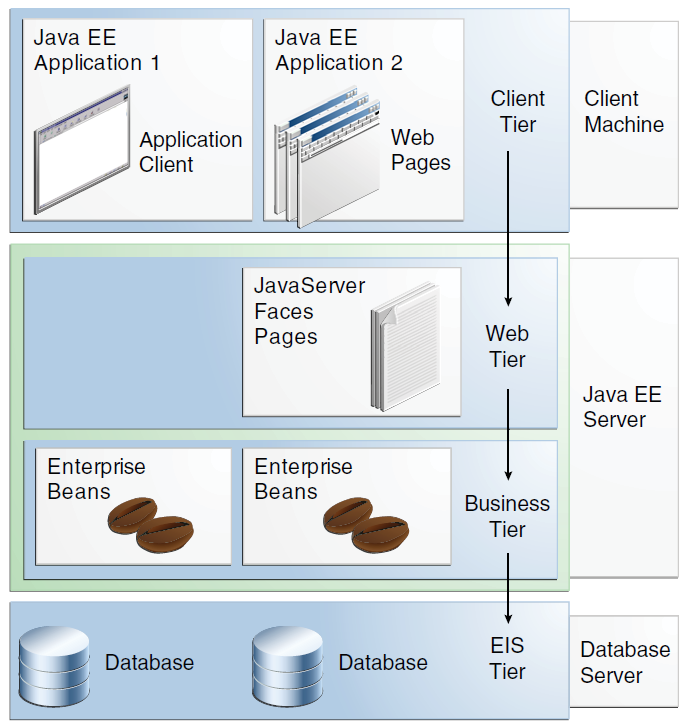
\includegraphics[width=\linewidth]{./images/JEE-arch}
\caption[JEE architecture]{JEE achitecture}
\label{fig:JEE-arch}
\end{figure}

As shown in figure \ref{fig:JEE-arch} JEE is divided in four tier:
\begin{itemize}
\item Client tier: containing Application Client and Web Pages it is the layer that directly interacts with the actors. As our project will be a web application the client will use a web browser to access pages.
\item Web tier: it contains the dynamic web pages that needs to be elaborated. This tier receives the requests from the client tier and forwards the pieces of data collected to the business tier waiting for processed data to be sent (eventually formatted) to the client tier.
\item Business tier: it contains the Java Beans, which are the elements that control the business logic of the application.
\item EIS tier: it contains the data source. In our case it is the database allowed to store all the relevant data and to retrieve them.
\end{itemize}

\section{Identifying sub-systems}
At this phase of the project we adopt a top-down approach to identify the main components of the system, once identified the sub-systems we will use a bottom-up approach to create more reusable components. We start by diving our system into smaller sub systems in order to better identify the various groups of functionalities and their interactions.

As depicted in figure \ref{fig:subsystems} the system is divided into three main packages, each with his own sub systems:
\begin{itemize}
\item User interface:
\begin{itemize}
\item Login page
\item Sign up page
\item Calendar page
\item Search page
\item Notification viewer
\end{itemize}

\item Business logic:
\begin{itemize}
\item Login manager
\item Sign up manager
\item Calendar manager
\item Search manager
\item Notification manager
\item Forecast manager
\end{itemize}

\item Persistence:
\begin{itemize}
\item Entity manager
\end{itemize}
\end{itemize}

\begin{figure}[h]
\centering
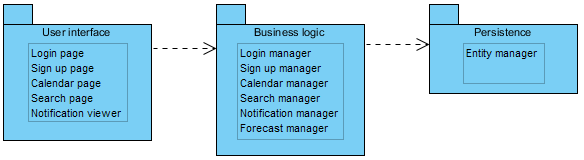
\includegraphics[width=\linewidth]{./images/sub-systems}
\caption[Subsystems]{System's packages and main components}
\label{fig:subsystems}
\end{figure}

\clearpage
\part{Persistent data management}
\section{Conceptual design}
\section{Logical design}
\subsection{ER restructuration}
RESTRUCTURATION IN INGLESE NON ESISTE
\subsection{Translation to logical model}

\clearpage
\part{User Experience}
\section{UX1}
\section{UX...n}

\clearpage
\part{BCE diagrams}
\section{Entity overview}
\section{BCE 1}
\section{BCE...n}
\section{User}
\subsection{BCE u1}
\subsection{BCE u...n}

\clearpage
\part{Sequence diagrams}
\section{SD1}
\section{SD..n}

\clearpage
\part{Final considerations}

\clearpage
\tableofcontents
\end{document}